\documentclass{report}
\usepackage{graphicx, tikz-cd, float, titlepic, booktabs} % Required for inserting images
\usepackage{pgfplots}
\usepackage{multicol}
\usepackage{makecell}
\pgfplotsset{compat=1.15}
\usepackage{mathrsfs}
\usetikzlibrary{arrows}
\usepackage{amsmath, amssymb, amsthm, amsfonts, siunitx, physics, gensymb}
\AtBeginDocument{\RenewCommandCopy\qty\SI}
\usepackage[version=4]{mhchem}
\usepackage[most,many,breakable]{tcolorbox}
\usepackage{xcolor, fancyhdr, varwidth}
\usepackage[Glenn]{fncychap}
%Options: Sonny, Lenny, Glenn, Conny, Rejne, Bjarne, Bjornstrup
\usepackage{hyperref, cleveref}
\usepackage{icomma, enumitem} %comma as decimal and continue enumerate with [resume]
\usepackage{plimsoll} %use standard state symbol with \stst
\usepackage[danish]{babel}
\usepackage{halloweenmath}
\renewcommand{\cellalign}{cl}
\renewcommand{\theadalign}{cl}
\renewcommand\theadfont{\bfseries}
%%%%%%%%%%%%%%%%%%%%%%%%%%%%%%
% SELF MADE COLORS
%%%%%%%%%%%%%%%%%%%%%%%%%%%%%%
\definecolor{myg}{RGB}{56, 140, 70}
\definecolor{myb}{RGB}{45, 111, 177}
\definecolor{myr}{RGB}{199, 68, 64}
\definecolor{mytheorembg}{HTML}{F2F2F9}
\definecolor{mytheoremfr}{HTML}{00007B}
\definecolor{mylenmabg}{HTML}{FFFAF8}
\definecolor{mylenmafr}{HTML}{983b0f}
\definecolor{mypropbg}{HTML}{f2fbfc}
\definecolor{mypropfr}{HTML}{191971}
\definecolor{myexamplebg}{HTML}{F2FBF8}
\definecolor{myexamplefr}{HTML}{88D6D1}
\definecolor{myexampleti}{HTML}{2A7F7F}
\definecolor{mydefinitbg}{HTML}{E5E5FF}
\definecolor{mydefinitfr}{HTML}{3F3FA3}
\definecolor{notesgreen}{RGB}{0,162,0}
\definecolor{myp}{RGB}{197, 92, 212}
\definecolor{mygr}{HTML}{2C3338}
\definecolor{myred}{RGB}{127,0,0}
\definecolor{myyellow}{RGB}{169,121,69}
\definecolor{myexercisebg}{HTML}{F2FBF8}
\definecolor{myexercisefg}{HTML}{88D6D1}
%%%%%%%%%%%%%%%%%%%%%%%%%%%%%%%%%%%%%%%%%%%%%%%%%%%%%%%%%%%%%%%%%%%%%%
% Box environments for theorems and problems
%%%%%%%%%%%%%%%%%%%%%%%%%%%%%%%%%%%%%%%%%%%%%%%%%%%%%%%%%%%%%%%%%%%%%
\setlength{\parindent}{1cm}
%================================
% Question BOX
%================================
\newtcbtheorem[]{question}{Opgave}{enhanced,
	before skip=2mm,after skip=2mm, colback=red!5,colframe=red!80!black,boxrule=0.5mm,
	attach boxed title to top left={xshift=1cm,yshift*=1mm-\tcboxedtitleheight}, varwidth boxed title*=-3cm,
	boxed title style={frame code={
					\path[fill=tcbcolback]
					([yshift=-1mm,xshift=-1mm]frame.north west)
					arc[start angle=0,end angle=180,radius=1mm]
					([yshift=-1mm,xshift=1mm]frame.north east)
					arc[start angle=180,end angle=0,radius=1mm];
					\path[left color=tcbcolback!60!black!65!red,right color=tcbcolback!60!black!65!red,
						middle color=tcbcolback!80!black!65!red!1!red]
					([xshift=-2mm]frame.north west) -- ([xshift=2mm]frame.north east)
					[rounded corners=1mm]-- ([xshift=1mm,yshift=-1mm]frame.north east)
					-- (frame.south east) -- (frame.south west)
					-- ([xshift=-1mm,yshift=-1mm]frame.north west)
					[sharp corners]-- cycle;
				},interior engine=empty,
		},
	fonttitle=\bfseries,
	title={#2},#1}{def}


\makeatletter
\newtcbtheorem{Question}{Opgave}{enhanced,
	breakable,
	colback=white,
	colframe=myb!80!black,
	attach boxed title to top left={yshift*=-\tcboxedtitleheight},
	fonttitle=\bfseries,
	title={#2},
	boxed title size=title,
	boxed title style={%
			sharp corners,
			rounded corners=northwest,
			colback=tcbcolframe,
			boxrule=0pt,
		},
	underlay boxed title={%
			\path[fill=tcbcolframe] (title.south west)--(title.south east)
			to[out=0, in=180] ([xshift=5mm]title.east)--
			(title.center-|frame.east)
			[rounded corners=\kvtcb@arc] |-
			(frame.north) -| cycle;
		},
	#1
}{def}
\makeatother
%================================
% DEFINITION BOX
%================================

\newtheorem{defin}{Definition}[section] % Creates a new counter, number within section

\newtcbtheorem[number within=section, use counter*=defin]{Definition}{Definition}{enhanced,
	before skip=2mm,after skip=2mm, colback=red!5,colframe=red!80!black,boxrule=0.5mm,
	attach boxed title to top left={xshift=1cm,yshift*=1mm-\tcboxedtitleheight}, varwidth boxed title*=-3cm,
	boxed title style={frame code={
					\path[fill=tcbcolback]
					([yshift=-1mm,xshift=-1mm]frame.north west)
					arc[start angle=0,end angle=180,radius=1mm]
					([yshift=-1mm,xshift=1mm]frame.north east)
					arc[start angle=180,end angle=0,radius=1mm];
					\path[left color=tcbcolback!60!black,right color=tcbcolback!60!black,
						middle color=tcbcolback!80!black]
					([xshift=-2mm]frame.north west) -- ([xshift=2mm]frame.north east)
					[rounded corners=1mm]-- ([xshift=1mm,yshift=-1mm]frame.north east)
					-- (frame.south east) -- (frame.south west)
					-- ([xshift=-1mm,yshift=-1mm]frame.north west)
					[sharp corners]-- cycle;
				},interior engine=empty,
		},
	fonttitle=\bfseries,
	title={#2},#1}{def}

\newtcbtheorem[number within=section]{definition}{Definition}
{%
	enhanced,
	breakable,
	colback = red!5,
	frame hidden,
	boxrule = 0sp,
	borderline west = {2pt}{0pt}{solid, red!75!black},
	sharp corners,
	detach title,
	before upper = \tcbtitle\par\smallskip,
	coltitle = red!75!black,
	fonttitle = \bfseries\sffamily,
	description font = \mdseries,
	separator sign none,
	segmentation style={solid, red!75!black},
}
{th}

\newtcbtheorem{theo}%
    {Theorem}{}{theorem}
\newtcolorbox{prob}[1]{colback=red!5!white,colframe=red!50!black,fonttitle=\bfseries,title={#1}}

%================================
% NOTE BOX
%================================

\usetikzlibrary{arrows,calc,shadows.blur}
\tcbuselibrary{skins}
\newtcolorbox{note}[1][]{%
	enhanced jigsaw,
	colback=gray!20!white,%
	colframe=gray!80!black,
	size=small,
	boxrule=1pt,
	title=\textbf{Note:},
	halign title=flush center,
	coltitle=black,
	breakable,
	drop shadow=black!50!white,
	attach boxed title to top left={xshift=1cm,yshift=-\tcboxedtitleheight/2,yshifttext=-\tcboxedtitleheight/2},
	minipage boxed title=1.5cm,
	boxed title style={%
			colback=white,
			size=fbox,
			boxrule=1pt,
			boxsep=2pt,
			underlay={%
					\coordinate (dotA) at ($(interior.west) + (-0.5pt,0)$);
					\coordinate (dotB) at ($(interior.east) + (0.5pt,0)$);
					\begin{scope}
						\clip (interior.north west) rectangle ([xshift=3ex]interior.east);
						\filldraw [white, blur shadow={shadow opacity=60, shadow yshift=-.75ex}, rounded corners=2pt] (interior.north west) rectangle (interior.south east);
					\end{scope}
					\begin{scope}[gray!80!black]
						\fill (dotA) circle (2pt);
						\fill (dotB) circle (2pt);
					\end{scope}
				},
		},
	#1,
}
%================================
% EXAMPLE BOX
%================================
\newtcbtheorem[number within=section, use counter from=definition]{Example}{Example}
{%
	colback = myexamplebg
	,breakable
	,colframe = myexamplefr
	,coltitle = myexampleti
	,boxrule = 1pt
	,sharp corners
	,detach title
	,before upper=\tcbtitle\par\smallskip
	,fonttitle = \bfseries
	,description font = \mdseries
	,separator sign none
	,description delimiters parenthesis
}
{ex}
%================================
% THEOREM BOX
%================================

\tcbuselibrary{theorems,skins,hooks}
\newtcbtheorem[number within=section, use counter from=definition]{Theorem}{Theorem}
{%
	enhanced,
	breakable,
	colback = mytheorembg,
	frame hidden,
	boxrule = 0sp,
	borderline west = {2pt}{0pt}{mytheoremfr},
	sharp corners,
	detach title,
	before upper = \tcbtitle\par\smallskip,
	coltitle = mytheoremfr,
	fonttitle = \bfseries\sffamily,
	description font = \mdseries,
	separator sign none,
	segmentation style={solid, mytheoremfr},
}
{th}

%%%%%%%%%%%%%%%%%%%%%%%%%%%%%%%%%%%%%%%%%%%%%%%%%%%%%%%%%%%%%%%%%
% SELF MADE COMMANDS
%%%%%%%%%%%%%%%%%%%%%%%%%%%%%%
\newcommand{\sol}{\setlength{\parindent}{0cm}\textbf{\textit{Løsning:}}\setlength{\parindent}{1cm}}
%%%%%%%%%%%%%%%%%%%%%%%%%%%%%%%%%
\usepackage[tmargin=2cm,rmargin=1in,lmargin=1in,margin=0.85in,bmargin=2cm,footskip=.2in]{geometry}\pagestyle{fancy}
\lhead{Minrui Kevin Zhou 3.b $\bigpumpkin$}
\rhead{Elektriske køretøjer $\mathghost$}

\title{
\[
\mathwitch*
\]
Elektriske køretøjer\\
{\Large \textbf{3.b fysik A}}}
\author{Kevin Zhou}
\date{\today}

\begin{document}
\maketitle
\begin{note}
  Databog fysik kemi (2007) er benyttet ved beregningerne. $\mathbat$
\end{note}
\begin{question}{Elfærge}{}
  Batteriet på elfærgen Aurora har det maksimale energiindhold 4160 kWh.
Mens færgen er i havn, oplades batteriet i 7,5 minutter med effekten 10,5
MW.
Spændingsfaldet under opladningen er det samme som batteriets nominelle
spændingsfald.
\begin{itemize}
  \item[a.] Beregn ændringen i batteriets ladningstilstand under opladningen.
\end{itemize}
Færgens batteri er opbygget af en række parallelkoblede strenge, hvor hver
streng består af 192 seriekoblede elementer. Hvert element har
hvilespændingen 3,9 V.
Under sejlads aflades batteriet med strømstyrken 112 A, og nyttevirkningen
af batteriet er 98 \%.
\begin{itemize}
  \item[b.] Bestem den indre resistans i færgens batteri.
\end{itemize}
\end{question}
\sol \\
\textbf{a.}
Siden effekten $P$ er konstant under opladningen, så må ændringen i ladningstilstand være 
\begin{equation*}
\begin{split}
  \Delta SoC&=\frac{P \cdot \Delta t}{E _{\text{max} }}\\
  &=\frac{10,5 \cdot 10^6 \;\unit{W} \cdot 7,5 \;\unit{min} }{4160 \cdot 10^3 \;\unit{W} \cdot 60 \;\unit{min} }\\
  &\approx 0,32\\
  &=32 \%.
\end{split}
\end{equation*}
Ændringen i batteriets ladningstilstand under opladningen må da være 32 \%.\\[1ex]
\textbf{b.}
Siden strengene af seriekoblede elementer er parallelkoblede, så må der gælde, at den samlede hvilespænding må være
\begin{equation*}
\begin{split}
  U_0&=U_0(\text{streng 1}) = U_0(\text{streng 2}) = \cdots =U_0(\text{streng } n)\\
  &=192 \cdot 3,9 \;\unit{V},
\end{split}
\end{equation*}
fordi hver streng består af 192 seriekoblede elementer, der hver har hvilespænding på 3,9 V.

Imidlertid har vi, at
\begin{equation*}
\begin{split}
  \eta =1-\frac{R_i \cdot I}{U_0} \iff R_i =\frac{(1-\eta) \cdot U_0}{I}.
\end{split}
\end{equation*}
Vi indsætter da de kendte værdier og får
\begin{equation*}
\begin{split}
  R_i &=\frac{(1-\eta) \cdot U_0}{I}\\
  &=\frac{(1-0,98)\cdot 192 \cdot 3,9 \;\unit{V} }{112 \;\unit{A} }\\
  &\approx 0,13 \;\unit{\ohm}. 
\end{split}
\end{equation*}
Den indre resistans i færgens batteri er altså $0,13 \;\unit{\ohm}$.

\begin{question}{Opladning af batteri}{}
Et batteri har den indre modstand $0,090 \;\unit{\ohm}$ og hvilespændingen 4,2 V.
\begin{itemize}
  \item[a.] Beregn den maksimale effekt, hvormed batteriet kan afgive energi under afladning.
\end{itemize}
Under opladning af et helt afladet batteri måles strømstyrken $I$ igennem
batteriet som funktion af tiden $t$.
Efter 2,5 h er batteriet fuldt opladet.
\begin{itemize}
  \item[b.] Bestem den tid, det tager at oplade batteriet til ladningstilstanden 90 \%.
\end{itemize}
\end{question}
\sol \\
\textbf{a.}
Den maksimale effekt må være
\begin{equation*}
\begin{split}
  P _{\text{max} }&=\frac{U_0^2}{4 \cdot R_i}\\
  &=\frac{\left(4,2 \;\unit{V} \right) ^2}{4 \cdot 0,090 \;\unit{\ohm}}\\
  &=49 \;\unit{W}.
\end{split}
\end{equation*}
Den maksimale effekt, hvormed batteriet kan afgive energi under afladning er altså $49 \;\unit{W}$.\\[1ex]
\textbf{b.}
Der gælder, at
\[
\Delta Q= \int_{t_1}^{t_2} I \,dt. 
\] 
Vi indsætter derfor de givne data i Logger Pro og finder arealet under $(t, I)$-grafen fra $t=0 \;\unit{h} $ til $t=2,5 \;\unit{h}$, som må svare til batteriets maksimale ladningskapacitet $Q _{\text{max} }$ (se \cref{fig:batteri}).
Vi får fra den numeriske integration, at
\[
Q _{\text{max} }=0,8042 \;\unit{A \cdot h}.
\] 
Vi kan nu udregne, hvilken ladningsmængde $Q_t$ batteriet har, når $SoC_t=90 \%$:
\begin{equation*}
\begin{split}
  Q_t &= SoC_t \cdot Q _{\text{max} }\\
  &= 0,9 \cdot 0,8042 \;\unit{A \cdot h} \\
  &\approx 0,7238 \;\unit{A \cdot h}. 
\end{split}
\end{equation*}
Fra \cref{fig:batteri} ser vi, at dette netop er tilfældet, når $t=1,04 \;\unit{h}$.
Altså tager det $1,04 \;\unit{h}$ at oplade batteriet til ladningstilstanden 90 \%.
\begin{figure}[H]
\begin{center}
  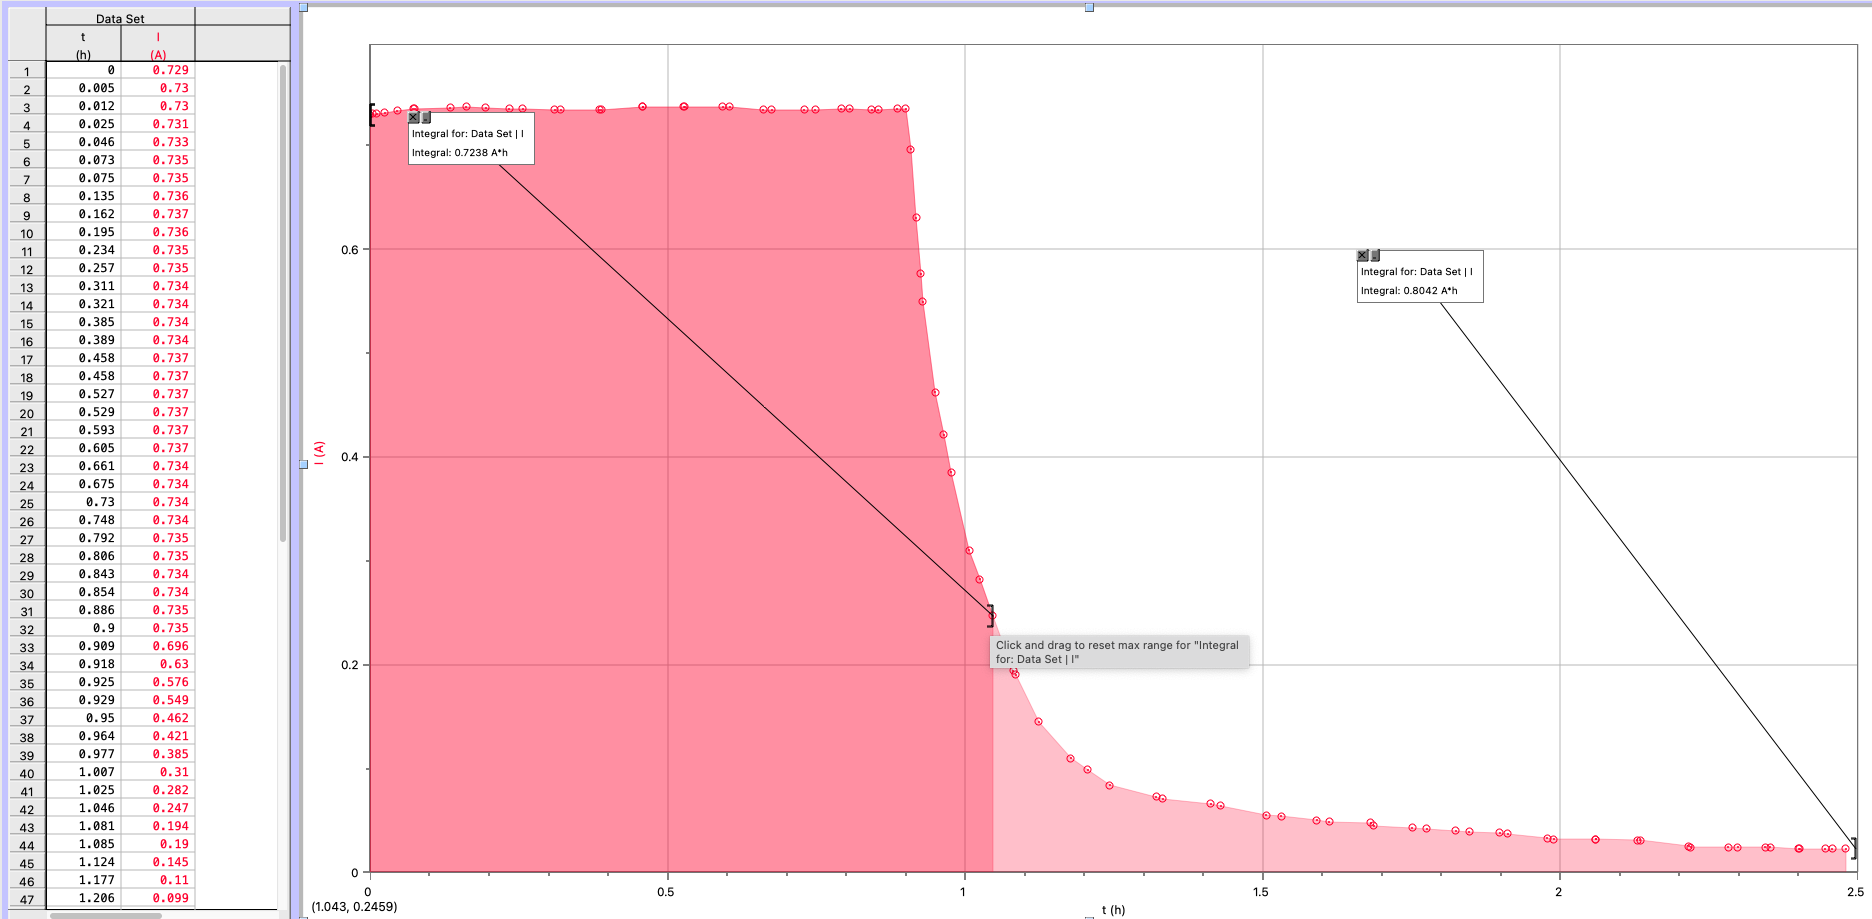
\includegraphics[width=0.8\textwidth]{batteri.png}
\end{center}
  \caption{Numerisk integration på $(t,I)$-grafen}
\label{fig:batteri}
\end{figure}

\end{document}
